
\section{Methodology \& Implementation}

IAM emission results are provided along a number of different dimensions,
including, temporal (normally half decade or decade), spatial (i.e., model
regions), gas species, and sectoral. Each individual temporal trajectory (i.e.,
unique combinations of regions, species, and sectors) must be harmonized to the
initial time period. Given a model trajectory, $m_{r, g, s}(t)$, historical
trajectory, $h_{r, g, s}(t)$, and initial time period $t_i$, a harmonized
trajectory can be calcluated.

In previous studies, two \textit{families} of methods have been used: those that
operate on the ratio of base year values (i.e., $\frac{h(t_i)}{m(t_i)}$) and
those that operate on the offset of base year values (i.e., $h(t_i) -
m(t_i)$). The \code{aneris} code base provides a number of variations on the
classic methods, including ratio-convergence methods shown in Equation
\ref{eqs:ratio}, offset-convergence methods shown in Equation \ref{eqs:offset},
and interpolation methods shown in Equation \ref{eqs:interpolate}; the
convergence factor for associated methods is shown first in Equation
\ref{eqs:factor}. Each is a function of time, model trajectory, historical
trajectory, harmonization time period, and a convergence time period ($t_f$),
where the harmonized trajectory converges to the unharmonized trajectory.

\begin{equation}\label{eqs:factor}
  \beta(t, t_i, t_f) =
  \begin{cases}
    1 - \frac{t - t_i}{t_f - t_i},& \text{if } t \leq t_f\\
    0,                        & \text{otherwise}
  \end{cases}
\end{equation}

\begin{equation}\label{eqs:ratio}
  m^{rat}(t, m, h, t_i, t_f) = [\beta(t, t_i, t_f) (\frac{h(t_i)}{m(t_i)} - 1) + 1] m(t)
\end{equation}

\begin{equation}\label{eqs:offset}
  m^{off}(t, m, h, t_i, t_f) = \beta(t, t_i, t_f) (h(t_i) - m(t_i)) + m(t)
\end{equation}
  
\begin{equation}\label{eqs:interpolate}
  m^{int}(t, m, h, t_i, t_f) =
  \begin{cases}
    \frac{m(t_f) - h(t_i)}{t_f - t_i}(t - t_i) + h(t_i), & \text{if } t \leq t_f\\
    m(t), & \text{otherwise}
  \end{cases}
\end{equation}

While historically expert opinion has guided the determination of harmonization
methods to choose for a given trajectory, a new, \textit{decision tree} approach
has been implemented in this work. In order to provide reasonable
\textit{default} methods, the historical trajectory, unharmonized model
trajectory, and relative difference between history and model values in the
harmonization year are analyzed. A figure of the decision tree used in this
analysis is shown in Figure \ref{}. 

% decision tree figure

A number of characteristics impact the decision of which default method to
select based on the effect of the characteristic on the potential harmonized
trajectory. For example, it is possible for models to report zero values in the
harmonization year in situations in which technologies are introduced in future
time periods in regions or for sectors which produce an emissions species that
is absent in the initial modeling period. In such cases, an offset method is
required as a ratio method would mask future emissions and erroneously harmonize
the trajectory. 

Variability of the historical trajectory is also an important characteristic
when considering the choice of harmonization method. Such trajectories are
normally indicative of emissions from land use sectors. Land use sectors are
modeled with varying fidelity by IAMs, but in general proxies are used for
emissions trajectories. Take for example the emissions of black carbon (BC) from
grassland burning in Africa \TODO{check that this is a good sector}: for most
models, the use of grass and paturelands is modeled, and the emissions of
species from the burning of these lands is determined by applying a emissions
factor to a proxy model of burning of these lands; in general, the more
grassland usage occurs, the higher the emissions from burning of
grasslands. Therefore, consistency in harmonization method is important due to
the approaches taken in modeling these sectors by IAMs. In order to reliably
detect land-use-like emissions, a measure of the covariance of the historical
trajectory is calculated as shown in Equation \ref{eqs:cov} and tested against a
threshold. To determine this threshold, an analysis of the recent CEDS
\TODO{cite ceds paper} historical data has been performed. Figure \ref{fig:cov}
shows the distribution of land-use covariances and non-land-use covariances as
determined for \TODO{list regions for 11 regions}. The minimum covariance
observed for land-use sectors is \TODO{find}, thus theshold used in this study
is \TODO{do this}. Notably, some non-land-use sectors , however,

\begin{equation}\label{eqs:cov}
    \Omega =  \frac{\sigma(h^{\prime}(t))}{\mu(h^{\prime}(t))}
\end{equation}


\begin{figure}
  \begin{center}
    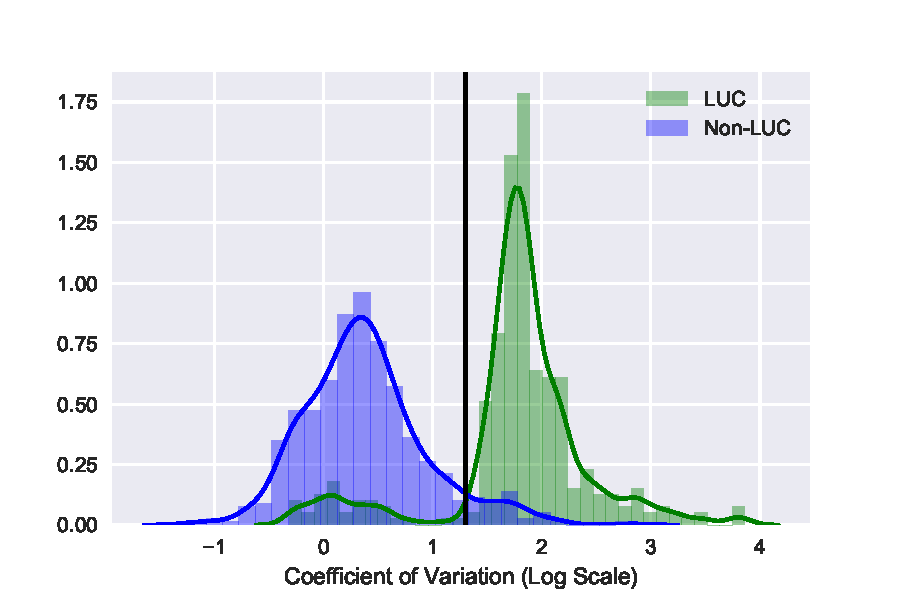
\includegraphics[width=\textwidth]{cov.pdf}
    \caption[]{
      \label{fig:cov}
      The distribution of $\Omega$ values for LUC and non-LUC historical
      trajectories are shown. The CEDS historical data is used for non-LUC data
      and \TODO{cite LUC data} is used for LUC data. All historical data has
      been aggregated to the 11-RCP \TODO{correct nomenclature?, cite} regions,
      and all gas species included in the historical datasets are included. The
      solid black line indicates the threshold value chosen in this analysis.
    }
  \end{center}
\end{figure}
